\documentclass{standalone}
\usepackage{tikz}

\begin{document}

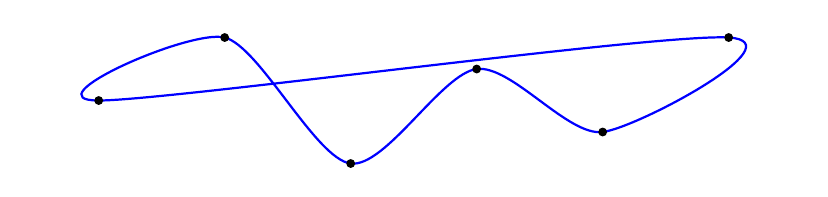
\begin{tikzpicture}[scale=0.8]
    % Define the points
    \coordinate (p1) at (0,0);
    \coordinate (p2) at (2,1);
    \coordinate (p3) at (4,-1);
    \coordinate (p4) at (6,0.5);
    \coordinate (p5) at (8,-0.5);
    \coordinate (p6) at (10,1);

    % Draw the smooth curve
    \draw[thick, blue] plot [smooth cycle] coordinates {
        (p1) (p2) (p3) (p4) (p5) (p6)
    };

    % Draw the dots
    \foreach \point in {p1, p2, p3, p4, p5, p6} {
        \fill (\point) circle (2pt);
    }
\end{tikzpicture}

\end{document}